\documentclass[sigconf,review,anonymous]{acmart}

\usepackage{xeCJK}
\setCJKmainfont{FandolSong-Regular}
\setCJKsansfont{FandolHei-Regular}
\usepackage{amsmath}
\usepackage{booktabs}
\usepackage{graphicx}
\usepackage{xcolor}
\usepackage{microtype}

\settopmatter{printacmref=true}
\acmConference[WWW '27]{The ACM Web Conference 2027}{May 10--14, 2027}{Dublin, Ireland}
\acmYear{2027}
\copyrightyear{2027}
\renewcommand\footnotetextcopyrightpermission[1]{}
\pagestyle{plain}
\graphicspath{{../../artifacts/www_revision/figures/}}

\IfFileExists{generated/results.tex}{
  % 本文件由 scripts/generate_paper_results.py 生成，请勿手工修改。
\newcommand{\DatasetCount}{11}
\newcommand{\AuditQueryCount}{90,000}
\newcommand{\AuditSampledConflictRate}{5.77}
\newcommand{\AuditConflictQuestionRate}{63.77}
\newcommand{\HistoricalLambdaZeroPRDelta}{-1.32}
\newcommand{\HistoricalTransferLambda}{0.1}
\newcommand{\HistoricalTransferReachDelta}{4.81}
\newcommand{\HistoricalTransferPRDelta}{-0.22}
\newcommand{\TunedReachDelta}{6.89}
\newcommand{\TunedReachCILow}{1.97}
\newcommand{\TunedReachCIHigh}{14.41}
\newcommand{\TunedPRDelta}{-0.57}
\newcommand{\TunedPRCILow}{-1.12}
\newcommand{\TunedPRCIHigh}{-0.17}
\newcommand{\TunedVsRandomReachDelta}{6.65}
\newcommand{\TunedVsRandomReachCILow}{1.75}
\newcommand{\TunedVsRandomReachCIHigh}{14.26}
\newcommand{\TunedVsRandomPRDelta}{-0.55}
\newcommand{\TunedVsRandomPRCILow}{-1.09}
\newcommand{\TunedVsRandomPRCIHigh}{-0.15}
\newcommand{\MaskSelectedDomainCount}{10}
\newcommand{\InteriorSelectedDomainCount}{1}
\newcommand{\BaselineSelectedDomainCount}{0}
\newcommand{\PRGuardrailViolationCount}{2}
\newcommand{\LambdaConflictRho}{-0.20}
\newcommand{\LambdaConflictP}{0.555}

}{
  \PackageError{path-supervision}{缺少 generated/results.tex}{请先运行 make paper-results；禁止使用占位实验数字。}
}

\title{单路径弱监督并不等于确定负例：超图检索中的路径一致负例重加权}
\ccsdesc[500]{Information systems~Retrieval models and ranking}
\ccsdesc[300]{Information systems~Question answering}
\keywords{图检索，超图，弱监督，负采样，检索增强生成，路径监督}

\begin{document}
\maketitle

\section{引言}

检索增强生成（retrieval-augmented generation, RAG）把外部证据检索与生成模型结合，使知识更新、证据追踪和长尾事实访问不再完全依赖参数记忆\cite{lewis2020rag}。当知识以图或超图组织时，检索器还需要在巨大的结构空间中选出可连接问题实体与答案的紧凑证据子图\cite{sun2019pullnet,zhang2022subgraph,he2024gretriever,lien2026hyperrag}。真实训练数据却很少提供逐步检索标签；常见做法是先从主题实体到答案实体选一条最短路径，再把该路径上的转移视为正例，把其余采样候选视为负例。

这种弱监督隐含了一个过强假设：``未被选中''等于``确定无关''。然而最短路径通常不唯一。一个没有进入所选路径的候选转移，仍可能位于另一条主题---答案等长最短路径上。如果它恰好被负采样器选中，同一个结构事实便同时得到``能够组成最短答案路径''与``应被压低''两种冲突证据。我们把这种候选称为\emph{路径一致负例}。这里的``一致''只描述图结构，不宣称候选在语义上必然相关，也不把它直接改成正例。

本文研究一个最小干预：保留原二元标签、候选集、检索模型和推理过程不变，仅把路径一致负例的损失权重从 $1$ 调整为数据集级 $\lambda\in[0,1]$。$\lambda=1$ 精确恢复基线，$\lambda=0$ 等价于完全屏蔽这类负例，中间值则保留较弱的负向约束。每个数据集只在独立 selection split 上从冻结网格选择 $\lambda_D^*$，并用逐题等量的随机降权对照排除``只是少惩罚了一些负例''这一解释。

本文的贡献有三点：

\begin{itemize}
  \item 给出适用于有向 incidence graph 的完整主题---答案成对判据，并构造可逐题复核的结构冲突审计；
  \item 提出不增加模型参数、不改标签和推理的置信度加权目标，并证明两个端点分别等价于基线与正确归一化的屏蔽损失；
  \item 在 WikiTopics\_QE 的 \DatasetCount{} 个领域上采用预先冻结的数据划分、五个共享随机种子、匹配随机对照和逐题配对 bootstrap，区分覆盖收益、原路径排序代价与结构特异性。
\end{itemize}

\paragraph{与 Web 的相关性。}
Web 知识检索需要在多源、异构且关系高元的事实网络中学习可追踪的证据链。路径监督决定了哪些超边会被检索器保留，因而直接影响 Web 问答中的证据覆盖、错误传播和生成器可见上下文。本文处理的不是新的图推理骨干，而是 Web 图检索训练数据中可普遍出现的弱监督冲突。

\section{相关工作}

\subsection{RAG 与图结构检索}

稠密检索和 RAG 奠定了以可学习检索器访问外部证据的基础\cite{karpukhin2020dpr,lewis2020rag}。面向知识图谱问答，PullNet 迭代扩展与问题相关的子图\cite{sun2019pullnet}；可分离子图检索器进一步强调答案覆盖与噪声控制之间的张力\cite{zhang2022subgraph}。G-Retriever 将文本属性图上的检索表述为结构优化问题\cite{he2024gretriever}，SubgraphRAG 重新考察图结构和语言模型在知识图谱 RAG 中的分工\cite{li2025subgraphrag}。HyperRAG 则用超图保存不宜拆成二元边的高元事实，并在其检索训练中使用路径派生监督\cite{lien2026hyperrag}。本文聚焦于这类路径派生标签本身，而非引入新的检索或生成模块。

\subsection{不完整监督与困难负例}

正例---未标注学习指出，未观察到正标签并不自动构成可靠负标签\cite{elkan2008pu,kiryo2017nnpu}；去偏对比学习也显示假负例会扭曲表征目标\cite{chuang2020debiased}。超边预测中的困难负采样同样关注负例构造对训练信号的影响\cite{deng2026hns}。与这些一般方法不同，我们能够利用已知主题、答案及有向最短距离，对一类冲突候选给出确定的结构判据，并只校准其损失强度。

\subsection{路径监督}

已有工作从答案可达路径中构造检索监督，或显式学习更有信息量的路径\cite{zhang2022subgraph,cattaneo2025groundtruth,gao2026pathise}。本文的出发点更窄：当训练流程只选中一条最短路径时，其他等长最短路径不应被默认当作置信度为一的负证据。我们不主张``所有最短路径都应标正''，而把它保留为诊断性强标签对照。

\section{问题定义：路径监督冲突}

对问题 $q$，令 $S_q$ 和 $A_q$ 分别为主题实体集与答案实体集。高元事实在 incidence graph $I$ 中表示为事实节点；候选转移 $t=(v,e,u)$ 表示从实体 $v$ 进入事实 $e$，再到实体 $u$，因此消耗两条 incidence edge。令 $d_I(x,y)$ 为有向无权最短距离。

\begin{definition}[路径一致转移]
候选转移 $t=(v,e,u)$ 对问题 $q$ 路径一致，当且仅当
\begin{equation}
\exists(s,a)\in S_q\times A_q:\quad
d_I(s,v)+2+d_I(u,a)=d_I(s,a).
\label{eq:path-consistency}
\end{equation}
\end{definition}

式\eqref{eq:path-consistency}保证该有向转移位于至少一条完整的主题---答案最短路径上。只检查 $u$ 是否比 $v$ 更接近答案并不充分，因为到达 $v$ 的前缀可能已经绕远。对实际进入训练的采样负例集合 $N_q$，定义冲突集合
\begin{equation}
D_q=\{t\in N_q:t\ \text{满足式}\eqref{eq:path-consistency}\}.
\end{equation}
这一定义不枚举全部组合候选，只判断真实进入损失的负例。

\begin{figure}[t]
  \centering
  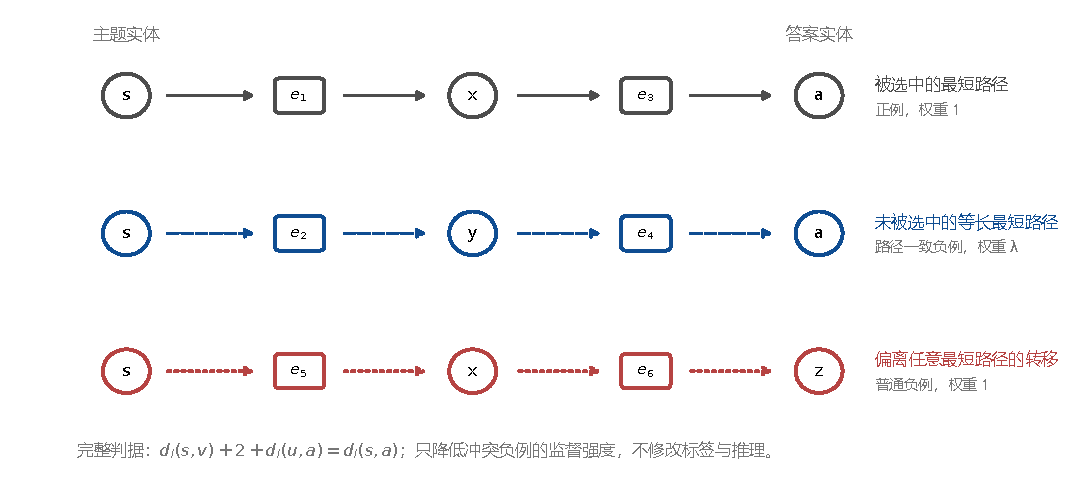
\includegraphics[width=\columnwidth]{method_overview.pdf}
  \Description{三行有向路径示意图：所选最短路径的正例权重为一，未选中的等长最短路径负例权重为 lambda，偏离最短路径的普通负例权重为一。}
  \caption{单路径弱监督产生的三类训练信号。未选中的等长最短路径具有结构冲突证据，本文保留其负标签但把损失权重降为 $\lambda$。}
  \label{fig:method}
\end{figure}

\section{置信度加权负监督}

\subsection{加权目标}

对训练候选 $i$ 的原标签 $y_i\in\{0,1\}$ 与模型 logit $z_i$，定义
\begin{equation}
w_i(\lambda)=
\begin{cases}
\lambda,& i\in D_q,\\
1,&\text{其他候选},
\end{cases}
\quad \lambda\in[0,1].
\end{equation}
一个 batch $B$ 的训练目标为
\begin{equation}
\mathcal L_B(\lambda)=
\frac{\sum_{i\in B}w_i(\lambda)\,
\operatorname{BCEWithLogits}(z_i,y_i)}
{\sum_{i\in B}w_i(\lambda)}.
\label{eq:weighted-loss}
\end{equation}
分母使用权重和而非 batch 大小，使 $\lambda=0$ 与删除 $D_q$ 后对剩余样本求均值严格等价；$\lambda=1$ 则与原 mean BCE 数值和梯度等价。该方法只增加一个数据集级超参数，不改变模型参数量、候选排序接口和推理开销。

\subsection{选择与识别对照}

每个领域在 $\{0,.1,.25,.5,.75,1\}$ 上独立选择 $\lambda_D^*$，唯一优化指标为 selection split 的 answer reach@10；精确并列时选择更大的 $\lambda$，即更弱干预。测试集在冻结前不可访问。

匹配随机降权对照对每个问题随机选择恰好 $|D_q|$ 个普通负例并赋予相同 $\lambda_D^*$。它保持被降权样本数与总损失质量变化相近，却删除路径信息。另设 all-shortest-positive 诊断，把 $D_q$ 改为正标签，用来检验结构一致是否足以支持强正监督；它不是本文方法。

\subsection{概念案例}

设主题实体为 $s$、答案实体为 $a$，图中有两条长度同为 $4$ 的最短路径：
\begin{align*}
s\rightarrow e_1\rightarrow x\rightarrow e_3\rightarrow a,\\
s\rightarrow e_2\rightarrow y\rightarrow e_4\rightarrow a.
\end{align*}
弱监督若只选择第一条路径，第二条上的 $(s,e_2,y)$ 仍可能被负采样。它满足
\[
d_I(s,s)+2+d_I(y,a)=0+2+2=4=d_I(s,a),
\]
所以属于 $D_q$。这并不证明 $e_2$ 的文本一定回答了问题；它只说明把该转移作为``确定负例''缺乏结构依据。直接标正可能过度承诺，完全屏蔽又可能丢失有用的排斥约束，因此中间权重提供了可验证的折中。

\section{实验设置}

\subsection{研究问题}

实验回答四个问题：RQ1，路径一致负例是否真实进入训练采样；RQ2，硬屏蔽与数据集级软加权如何影响答案覆盖和原路径排序；RQ3，收益是否来自路径信息而非等量随机降权；RQ4，最优权重是否随领域冲突率系统变化。

\subsection{数据、划分与模型}

我们使用 WikiTopics\_QE 的 \DatasetCount{} 个领域整数图。所有实验臂共享候选、特征和问题级 $60/10/15/15$ 训练/早停验证/选择/测试划分；划分种子为 20260920，采样与训练种子为 42--46。结构代理检索器由实体/关系嵌入和两层 MLP 构成。由于公开资产中缺少完整 NLG、构图后 GraphML、GTE 表示、官方检索器 checkpoint 与端到端生成配置，本稿明确把主实验限定为\emph{结构代理检索}，不把它写成官方 HyperRAG QA 复现。

\subsection{指标与统计}

主指标为 Top-10 转移能否连接主题与任一答案的 answer reach@10。次指标包括相对公开所选路径的 MRR/PR-AUC，以及相对全部最短路径转移的 MRR/PR-AUC。差值按 query key 严格配对，先在五个种子间等权平均，再做 10,000 次 paired bootstrap；跨领域结果以领域为等权单位。所有数值、表格和图均由聚合产物自动生成。

\section{结果}

\subsection{RQ1：冲突是否进入训练损失}

逐题审计覆盖 \AuditQueryCount{} 个问题。真实采样负例中有 \AuditSampledConflictRate\% 满足完整路径一致条件，至少一个随机种子采到冲突负例的问题占 \AuditConflictQuestionRate\%。这表明该现象不是只存在于组合候选空间的理论可能性，而会实际进入训练目标。图\ref{fig:conflict}区分了完整候选空间的稀疏比例、采样后的富集比例和受影响问题比例。

\begin{figure*}[t]
  \centering
  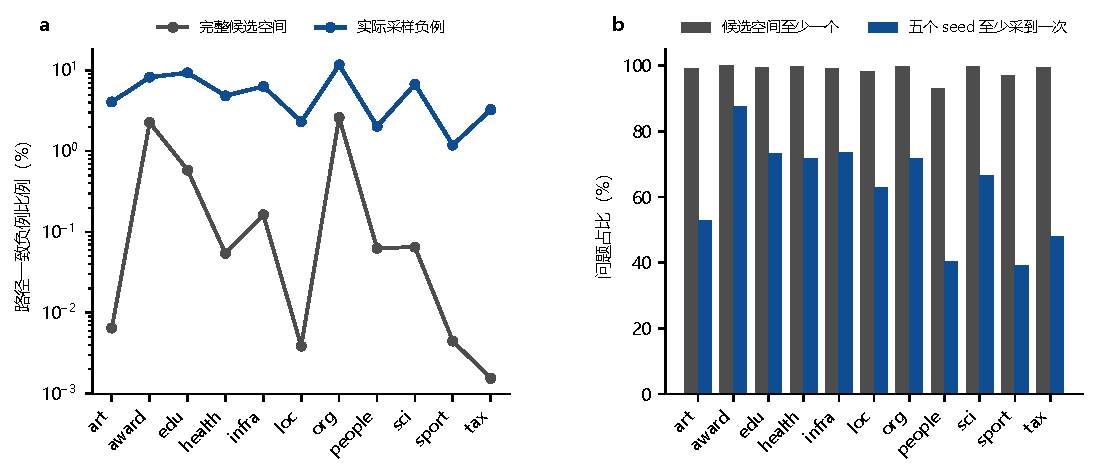
\includegraphics[width=0.92\textwidth]{path_conflict.pdf}
  \Description{十一领域候选空间、实际采样与受影响问题的路径冲突率对比。}
  \caption{RQ1：\DatasetCount{} 个领域的路径监督冲突。候选级比例与问题级覆盖采用不同面板，避免用总体均值掩盖分布。}
  \label{fig:conflict}
\end{figure*}

\begin{table*}[t]
  \centering
  \caption{逐领域结构代理测试结果。五个实验臂的数值均为 answer reach@10（\%），末列为加权相对基线的 selected-path PR-AUC 差值（百分点）；$\lambda_D^*$ 只由 selection split 冻结。}
  \label{tab:main}
  \resizebox{\textwidth}{!}{\begin{tabular}{lrrrrrrr}
\toprule
领域 & $\lambda_D^*$ & 基线 & 屏蔽 & 加权 & 随机 & 全部标正 & $\Delta$PR-AUC \\
\midrule
art & 0.00 & 85.65 & 88.12 & 88.12 & 86.09 & 87.96 & -0.00 \\
award & 0.00 & 79.59 & 93.99 & 93.99 & 80.99 & 96.41 & -0.97 \\
edu & 0.00 & 84.52 & 91.26 & 91.26 & 84.68 & 92.46 & -1.22 \\
health & 0.00 & 76.48 & 80.47 & 80.47 & 76.00 & 82.19 & -0.60 \\
infra & 0.00 & 91.14 & 92.64 & 92.64 & 91.25 & 92.96 & -0.26 \\
loc & 0.00 & 99.17 & 99.17 & 99.17 & 99.20 & 99.23 & -0.08 \\
org & 0.00 & 58.53 & 98.03 & 98.03 & 57.86 & 98.63 & -2.83 \\
people & 0.00 & 94.40 & 95.10 & 95.10 & 94.60 & 94.90 & -0.03 \\
sci & 0.00 & 84.07 & 88.36 & 88.36 & 84.81 & 89.11 & -0.34 \\
sport & 0.00 & 97.57 & 98.37 & 98.37 & 97.87 & 98.23 & +0.03 \\
tax & 0.10 & 85.17 & 87.00 & 86.55 & 85.57 & 88.07 & -0.01 \\
\bottomrule
\end{tabular}
}
\end{table*}

\subsection{RQ2：硬屏蔽还是软监督}

历史端点实验显示，$\lambda=0$ 使 selected-path PR-AUC 相对基线下降 \HistoricalLambdaZeroPRDelta{} 个百分点，超过预注册的一百分点保护线。因此，重复实验不能把这次已观察到的失败改写为成功；它只能估计不确定性。历史固定 $\lambda=\HistoricalTransferLambda$ 的跨领域迁移则使 answer reach@10 宏平均提高 \HistoricalTransferReachDelta{} 个百分点，同时 selected-path PR-AUC 变化 \HistoricalTransferPRDelta{} 个百分点，提示中间权重值得在严格独立划分上检验。

在新的数据集级选择协议下，$\lambda_D^*$ 相对 $\lambda=1$ 的宏平均 answer reach@10 差值为 \TunedReachDelta{} 个百分点（95\% CI [\TunedReachCILow, \TunedReachCIHigh]），selected-path PR-AUC 差值为 \TunedPRDelta{} 个百分点（95\% CI [\TunedPRCILow, \TunedPRCIHigh]）。表\ref{tab:main}报告逐领域结果，图\ref{fig:tradeoff}将覆盖收益与排序代价并列展示。

\begin{figure*}[t]
  \centering
  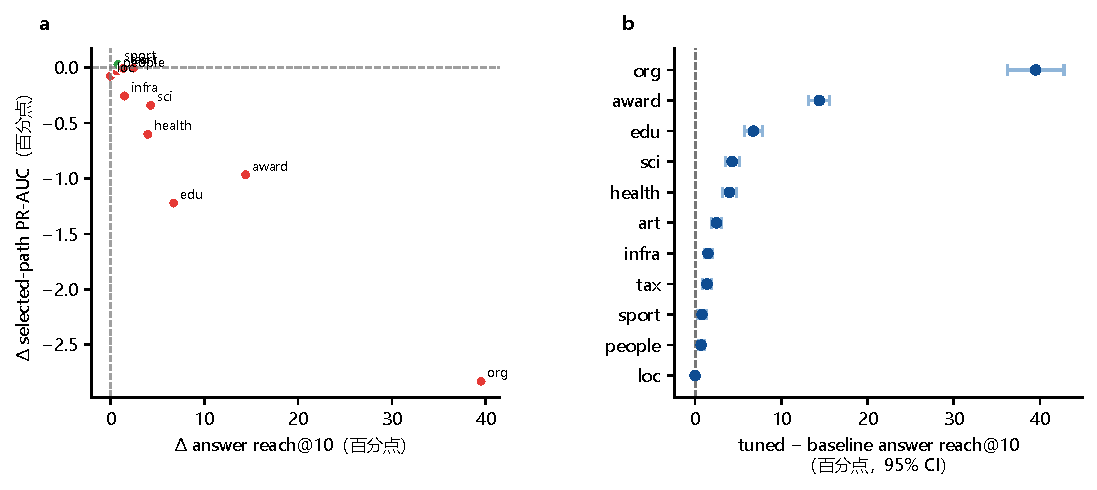
\includegraphics[width=0.92\textwidth]{coverage_ranking_tradeoff.pdf}
  \Description{逐领域覆盖变化与所选路径排序变化的散点图，以及带百分之九十五置信区间的森林图。}
  \caption{RQ2：冻结 $\lambda_D^*$ 相对基线的覆盖---排序权衡，以及逐领域 answer reach@10 配对区间。}
  \label{fig:tradeoff}
\end{figure*}

\subsection{RQ3：路径信息是否必要}

相对逐题匹配的随机降权，路径一致加权的宏平均 answer reach@10 差值为 \TunedVsRandomReachDelta{} 个百分点（95\% CI [\TunedVsRandomReachCILow, \TunedVsRandomReachCIHigh]）。该对照直接检验收益能否仅由降低若干负例权重解释。表\ref{tab:main}同时报告 all-shortest-positive；若强正标记不优于软加权，则结构可达性不足以替代语义相关性判断。

\subsection{RQ4：领域特异权重}

图\ref{fig:lambda}给出完整 selection 曲线、各领域冻结值及冲突率相关性。采样冲突率与 $\lambda_D^*$ 的 Spearman $\rho=\LambdaConflictRho$（$p=\LambdaConflictP$）。这是仅含 \DatasetCount{} 个领域的探索性分析，不作因果解释，也不据此修改冻结网格或删除不显著结果。

\begin{figure*}[t]
  \centering
  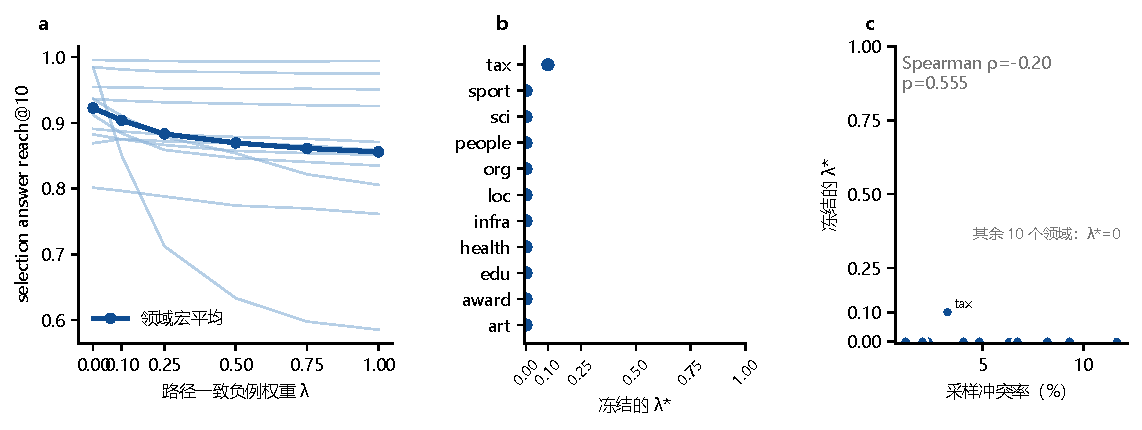
\includegraphics[width=0.96\textwidth]{lambda_sensitivity.pdf}
  \Description{选择集上的 lambda 灵敏度曲线、逐领域冻结 lambda 和冲突率相关性。}
  \caption{RQ4：selection 灵敏度、逐领域 $\lambda_D^*$ 与采样冲突率的探索性关系。}
  \label{fig:lambda}
\end{figure*}

\section{讨论与局限}

第一，路径一致是结构证据，不是语义标签。本文的语义审计协议要求两名真实标注者在盲化条件下独立判断``有用证据/语义不足/无法判断''，计算 Cohen's $\kappa$，分歧必须人工裁决；在完成前不报告虚构的语义比例。第二，当前主结果是结构代理检索器，而非官方 HyperRetriever 或端到端生成质量，因此结论限于监督冲突与结构检索行为。第三，$\lambda_D^*$ 是数据集级常数，不能适应单题置信度；这是为了保持方法可识别且不引入额外模型。第四，最短路径本身偏好短证据链，可能遗漏语义充分但更长的推理路径。

\section{结论}

单路径弱监督把一个可观测选择过程误当成了完整的负例标注。完整主题---答案距离判据能够定位真实进入损失的路径一致负例；数据集级 $\lambda$ 重加权则在不改模型、标签和推理的条件下校准其监督强度。本文的实证判断以冻结测试结果为准：覆盖收益必须同时对照原路径排序代价和等量随机降权，不能仅凭某一次指标提高宣称方法成功。

\bibliographystyle{ACM-Reference-Format}
\bibliography{references}

\appendix
\section{可复现性与历史 provenance}

历史 $\lambda=0$ 失败结果与固定 $\lambda=0.1$ 迁移结果均只读保留。新实验为每个作业记录实验 ID、UTC 时间、Git 提交和脏状态、完整命令、冻结配置、数据版本声明、随机种子、$\lambda$、骨干、GPU、Python/PyTorch/CUDA 版本、逐题指标与 checkpoint 指针。论文宏和表格只从聚合 JSON/CSV 生成；缺少正式产物时编译会失败而非使用占位数字。

\begin{table}[h]
  \centering
  \caption{逐领域路径冲突审计。}
  \resizebox{\columnwidth}{!}{\begin{tabular}{lrrr}
\toprule
领域 & 问题数 & 采样冲突率（\%） & 涉及冲突的问题（\%） \\
\midrule
art & 10,000 & 4.06 & 52.93 \\
award & 10,000 & 8.22 & 87.62 \\
edu & 10,000 & 9.33 & 73.27 \\
health & 10,000 & 4.85 & 71.77 \\
infra & 10,000 & 6.32 & 73.59 \\
loc & 4,000 & 2.32 & 62.80 \\
org & 4,000 & 11.67 & 71.73 \\
people & 10,000 & 2.02 & 40.48 \\
sci & 10,000 & 6.74 & 66.57 \\
sport & 4,000 & 1.19 & 39.10 \\
tax & 8,000 & 3.26 & 47.85 \\
\bottomrule
\end{tabular}
}
\end{table}

\begin{table*}[h]
  \centering
  \caption{selection split 上的 $\lambda$ 灵敏度（answer reach@10，百分数）。}
  \resizebox{\textwidth}{!}{\begin{tabular}{lrrrrrrr}
\toprule
领域 & $\lambda_D^*$ & 0 & .10 & .25 & .50 & .75 & 1.0 \\
\midrule
art & 0.00 & 89.08 & 88.68 & 88.23 & 87.86 & 87.58 & 87.08 \\
award & 0.00 & 93.63 & 91.05 & 87.89 & 85.37 & 82.17 & 80.57 \\
edu & 0.00 & 91.20 & 88.41 & 85.88 & 84.63 & 84.05 & 83.49 \\
health & 0.00 & 80.13 & 79.65 & 78.80 & 77.41 & 76.99 & 76.15 \\
infra & 0.00 & 93.64 & 93.38 & 93.13 & 92.92 & 92.69 & 92.56 \\
loc & 0.00 & 99.57 & 99.50 & 99.40 & 99.33 & 99.36 & 99.43 \\
org & 0.00 & 98.47 & 85.03 & 71.23 & 63.33 & 59.77 & 58.53 \\
people & 0.00 & 95.48 & 95.38 & 95.28 & 95.15 & 95.18 & 95.10 \\
sci & 0.00 & 88.23 & 87.50 & 86.63 & 85.74 & 85.39 & 85.14 \\
sport & 0.00 & 98.49 & 98.13 & 97.79 & 97.73 & 97.53 & 97.49 \\
tax & 0.10 & 86.90 & 87.55 & 87.20 & 86.92 & 86.57 & 85.83 \\
\bottomrule
\end{tabular}
}
\end{table*}

\end{document}
